\chapter{Justificación}
\label{Justificación}

En esta sección deben señalarse las razones, causas, argumentos de orden científico, metodológico por las cuales se realiza el proyecto de investigación. Como también debe explicar la trascendencia y utilidad teórica, práctica o metodológica que generará el trabajo y quiénes serán los beneficiarios de los productos  alcanzados. La redacción debe responder a la pregunta \textbf{¿Por qué investigar?}, puede referirse al interés por investigar el tema, a la novedad sobre el tema, su importancia  científica, impacto social o necesidad de resolver el problema \cite{herrera2004tutoria}.

Para su redacción, es recomendable hacer las siguientes preguntas:
\begin{enumerate}
    \item ¿Por qué se hace la investigación?
    \item ¿Cuáles serán sus aportes?
    \item ¿A quiénes pudiera beneficiar?
    \item ¿Cuál es el impacto y relevancia?
    \item ¿Cuál es la utilidad práctica?
\end{enumerate}

Además, \cite{hernandez2018metodologia} menciona 5 aspectos importantes en la Justificación, estos son:
\begin{enumerate}
    \item Conveniencia;
    \item Relevancia Social;
    \item Implicaciones prácticas;
    \item Valor Teórico, y;
    \item Utilidad Metodológica.
\end{enumerate}

La justificación debe ser argumentativa.(debe incluir citas bibliográficas).

\textbf{Ejemplos}
%La justificación pueden abarcar criterios como: científico, académico, social, técnico-tecnológico, ambiental y económico en su totalidad.

Criterios simples como: teórica, práctica y metodológica. 


\small{
\begin{itemize}
    \item[\textbf{A}] \footnote{Proyecto Smart Library UNL} Poseer una biblioteca inteligente en la Universidad es lo más idóneo, así los miembros (docentes, administrativos, estudiantes) tendrán la comodidad de trabajar o estudiar en un ambiente que llame aún más su atención.
    La biblioteca inteligente. sin duda alguna conlleva un trabajo de varios años e inversión de recursos para poder obtener un resultado tangible; por lo tanto este trabajo se enfoca en el desarrollo de un modelo que especifique los requerimientos para los servicios que preste la biblioteca como tal, el diseño del Sistema de Información (Administración, Organización, Tecnología: Software, Telecomunicaciones, etc.), y el estudio para la creación de una biblioteca inteligente.
    Para la idea propuesta, la UNL se encuentra en las posibilidades de brindar el apoyo necesario para que se lleve a cabo este trabajo; lo más importante es la oportunidad de contar con docentes experimentados en cada área específica necesarias para conjuntamente construir la propuesta que permite aplicar los conocimientos adquiridos durante los cinco años de formación profesional, aportando al campo científico y social con una solución innovadora sobre el problema detectado, con el fin de fomentar el uso de las TIC en la educación. 
    Tanto las herramientas necesarias en hardware y software son mínimas, y no presentan una inversión significativa en gran parte del proyecto, se tiene el factor económico necesario para sobrellevar esta idea; por otro lado, al ser un resultado intangible, no se hará uso de materiales que puedan presentar algún tipo de amenaza sobre el medio ambiente. 
    Este proyecto de Trabajo de Titulación, se ha formulado con el fin de desarrollar el estudio de factibilidad y viabilidad para la creación de una “Smart Library” en la Facultad de Energía; se enmarca en la SENESCYT priorizada sobre la línea de investigación de Ambientes Inteligentes; línea de investigación de la Carrera de Ingeniería en Sistemas de la Facultad de Energía las Industrias y los Recursos Naturales no Renovables de la Universidad Nacional de Loja. 
    \item[\textbf{B}] \footnote{Fuente: Universidad Continental}
   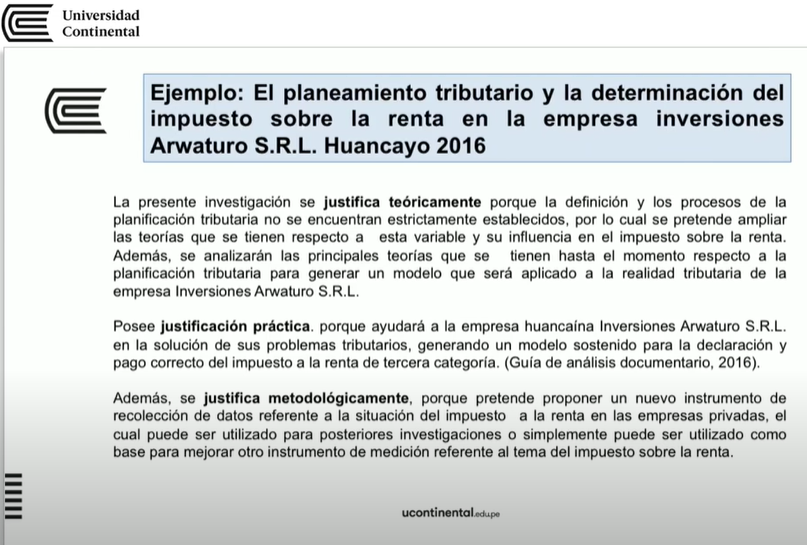
\includegraphics[scale=0.8]{img/ejempl2.png}
    
\end{itemize}
}

